\documentclass{article}
\usepackage[utf8]{inputenc}
\usepackage[margin=1in]{geometry}
\usepackage{graphicx}
\usepackage{natbib}
\usepackage{enumitem}
\usepackage{array}
\usepackage{gensymb}
\usepackage{indentfirst}
\graphicspath{ {Images/} }
\usepackage{float}
\usepackage[table,xcdraw]{xcolor}
\usepackage{amsmath}

\title{Physics 111A Fall 2016- Lab 11\\Signal Processing and Feedback Control}
\author{Joshua Levy\\Lab Partner: Alex Chuang}
\date{November 20th, 2016}

\begin{document}

\maketitle

\section{Lab Write Up}
%1
\subsection{Bandwidth Narrowing: Filters}
    My partner and I used the program Filter.vi and noticed the following effects:
    \begin{itemize}
        \item Studying the synchronicity of the filtered signal, we noticed that the modulation minima of filter signal occurred at same time as minima of unfiltered signal.
        \item Decreasing the bandpass so cutoff frequencies were at f = 75.5 Hz and f= 74.5 Hz, we see that the difference in time between minimum points is 0.6 seconds, with filtered signal occurring after unfiltered. Amplitude was same. So we see that decreasing the bandpass will also cause the filtered signal to become more asynchronous with the filtered signal.
        \item We narrowed our bandpass such that the cutoff frequencies were at 74.8Hz and 75.2Hz. At this bandpass, $\Delta$f = 0.4Hz, we saw that the amplitude of the signal was still close to one, and as we narrowed the bandpass from here, the signal began to decrease in amplitude. So this is the most narrow we can make the bandpass before the amplitude of the signal decreases.
        \item Changing the modulation frequency to 1, and we see that the narrowest bandpass that could occur before the amplitude decreases is at $f_{cutoff}$ = 73.5Hz, 76.5Hz ($\Delta$f = 3Hz), where the amplitude was just around 0.9 of the maximum.
        \item The minimum acceptable bandpass appears to become narrower with a lower modulation frequency.
        \item The scaling mentioned in the previous bullet point is can be explained by: as we decrease the modulation frequency, the amount of time by which you are sampling the signal effectively increases, and thus you can collect more data on the signal, thereby decreasing the bandpass of the filter. Another way of explaining this is through the Convolution Theorem \cite{conv}, which states that if you take the fourier transform of two signals being multiplied together (suppose this is our main signal f times the modulating signal g), the result is the fourier transform of f convoluted with the fourier transform of g. That is,
        \begin{equation}
            F\{fg\} = F\{f\}*F\{g\}
        \end{equation}
        where fg is the two signals multiplied together and * is the convolution operator. $F\{fg\}$ is the final output of our FFT of the main signal times the modulation signal. The convolution operator is effectively an integral transformation, and has the effect of narrowing the frequency response curve of f as the modulation frequency decreases.
    \end{itemize}

%2
\subsection{}
    We restored to the original parameters. We turned on 60Hz noise, and we saw that the unfiltered signal becomes hairy/choppy as the amplitude of the noise increases. The filtered signal is much more smoothed out, is less hairy than the original, and maintains the original amplitude of the signal. The 60 Hz noise appeared to be canceled by the bandpass filter. As we decrease the signal amplitude after narrowing our bandpass to the minimum values of [1.1], we can still kind of recover/notice the signal through the noise when the original signal is 0.03 amplitude before the 60Hz noise takes over (low signal to noise ratio). Thus, we also notice that the filter does a good job in removing the 60Hz noise.\\\indent The 60 Hz noise was approximately 1$V_{pp}$, and the signal was recoverable with a large enough signal to noise ratio.  
    
    
%3
\subsection{}
    See signature page
    
%4
\subsection{Bandwidth Narrowing: FFTs}
    With the given settings specified in the lab instructions, we displayed individual datapoints on an FFT graph with various signal frequencies. For a given signal frequency f, we were asked to find the width of the peak and how many points lay inside the frequencies specified by the peak. To do this, the width of our peak was defined by the full width at half max, that is, we found the max amplitude of the peak frequency (signal frequency), and found the "rolloff" frequencies (low $f_1$, high $f_2$) whose amplitude was -3dB from the peak. The width is:
    \begin{equation}
        \Delta f = f_2 - f_1
    \end{equation}
    We changed the signal frequency by increments of 0.01Hz. Below is a table of the data we found:
    \begin{table}[H]
        \centering
        \caption{Bandwidth across various signal frequencies and number of samples}
        \label{my-label}
        \begin{tabular}{llllll}
        \textbf{Number of Samples} & \textbf{f (Hz)} & \textbf{$f_2$ (Hz)} & \textbf{$f_1$ (Hz)} & \textbf{$\Delta f$ (Hz)} & \textbf{Points} \\ \hline
        10k & 75 & 75.045 & 74.95 & 0.095 & 1 \\
        10k & 75.01 & 75.064 & 74.97 & 0.094 & 1 \\
        10k & 75.02 & 75.08 & 74.97 & 0.11 & 1 \\
        10k & 75.03 & 75.1 & 74.97 & 0.13 & 2 \\
        10k & 75.04 & 75.11 & 74.97 & 0.14 & 2 \\
        10k & 75.05 & 75.12 & 74.98 & 0.14 & 2 \\
        20k & 75 & 75.027 & 74.97 & 0.057 & 1 \\
        30k & 75 & 75.018 & 74.983 & 0.035 & 1 \\
        40k & 75 & 75.02 & 74.99 & 0.03 & 1 \\
        50k & 75 & 75.01 & 74.99 & 0.02 & 1
        \end{tabular}
        \end{table}
    We see that given peak frequency of 75 Hz with 10k samples, the width of the peak is 0.095 Hz with 1 data point in between the frequency range that specifies the width of the peak. We can estimate the width of the peak by taking the fourier transform of the time domain data and finding the first zeroes. From the lab instruction sheet \cite{lab11}, we see that this occurs when our width $\Delta f$ is on the same order of magnitude as $\frac{1}{T}$, where T is the number of samples divided by the sampling rate. In this case, $\Delta f \approx \frac{1000}{10000}$Hz = 0.1 Hz, which is very close to the $\Delta f = 0.095Hz$ found in the table above for the same parameters. As we increase the signal frequency by 0.01Hz increments, we notice via the table above that the width of the peak ($\Delta f$) increases. As we increase the number of samples, we see that (above table) the width of the peak begins to decrease. At 20k samples, we expect the width ($\Delta f = \frac{sampling rate}{Number of Samples}$ to be $\frac{1000}{20k}*Hz$ = 0.05Hz, which is really close to expectation. At 30k samples, $\Delta f$ should be 0.0333 Hz, close to the one in the table, and at 50k samples, $\Delta f$ should be 0.02 Hz, which is pretty much the one on the table. So we see that our measured values conforms with expectations as we increase the number of samples.
    
%5
\subsection{}
    Using the same program with a sampling rate of 1k (and with newly specified settings), we see that the highest frequency plotted is at 500Hz. This is what we would expect because it is half of our sampling rate. We know that the sampling rate is at our nyquist frequency, the nyquist frequency being twice the highest signal present in the signal. We also know the nyquist frequency is the minimum frequency at which the signal can be sampled without introducing errors, and this should make 500 Hz be our maximum found frequency for the given sampling rate. As we increased the sampling rate to 2k, our max found frequency signal was 1kHz. As we increased the sampling rate to 3k, our max found frequency was 1.5 kHz. The highest frequency scales to half the sampling rate, seeming to affirm Nyquist's theorem.
    
%6
\subsection{}
    We set the 60 Hz Comb Amplitude to 1, and using the specified settings, we expanded the FFT axis to try to view the 75 Hz signal. At 10k samples with a 1k sampling rate, we brought the signal frequency to 60.4 Hz, only 0.4Hz away from the 60 Hz noise, and we were still able to distinguish the signal on a FFT plot. \\\indent We increased the number of samples to 20k, and this narrowed the peaks of the signal and the noise, so we were able to distinguish the signal at 60.2 Hz, only 0.2 Hz away from the noise. As we increased number of samples to 30k, our closest distinguishable frequency was at 60.13 Hz, only 0.13 Hz away from 60 Hz signal. We see that increasing the number of samples allows us to distinguish the signal at frequencies closer to the noise.
     
%7
\subsection{}
    Turning the 60Hz Comb off, setting the White Noise Amplitude to 1, and changing One Shot to Cycle Repetitively, and we see that we can pick out an 0.08 amplitude (75Hz) signal from the noise.
    
%8
\subsection{Averaging}
    See signature page

%9
\subsection{Pattern Matching}
    See signature page

%10
\subsection{Equivalent Time Sampling}
    See signature page

%11
\subsection{Dithering}
    See signature page

%12
\subsection{}
    We wrote the routine "Position Calibrator.vi" to calibrate a chart of ball position data with light level data. We actually modified the template, and below are images of our routine's construction:
    \begin{figure}[H]
        \centering
        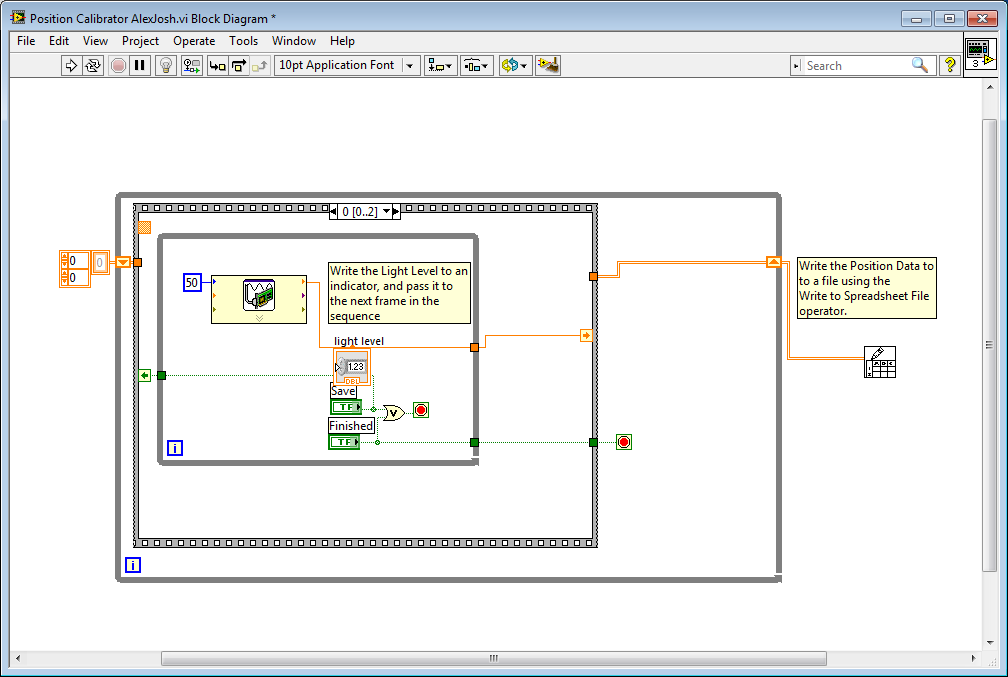
\includegraphics[scale = 0.3]{12a.PNG}
        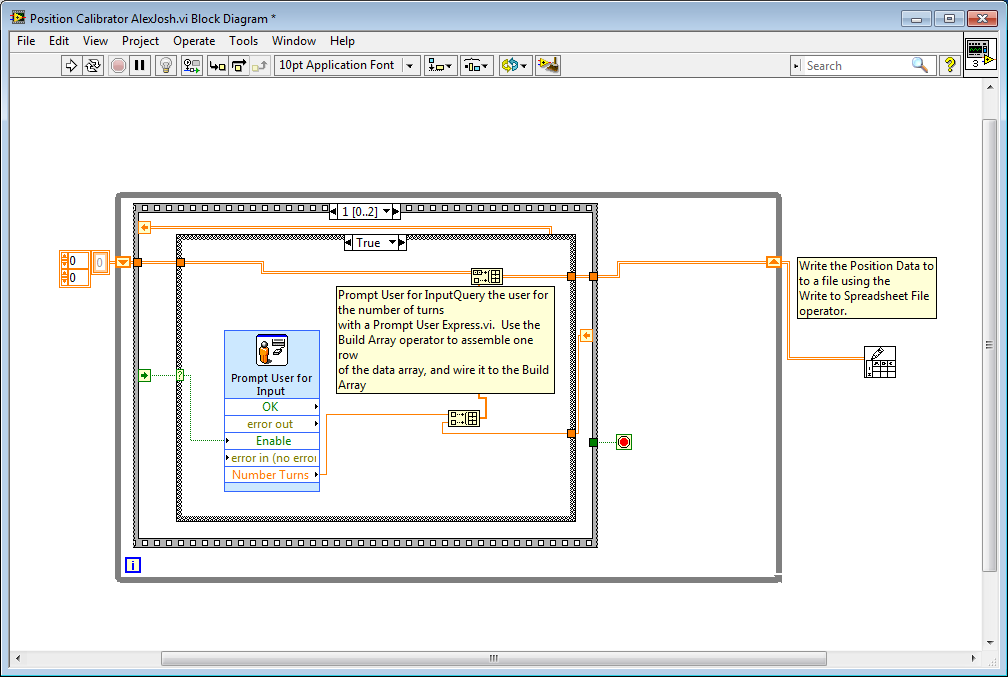
\includegraphics[scale = 0.3]{12b.PNG}
        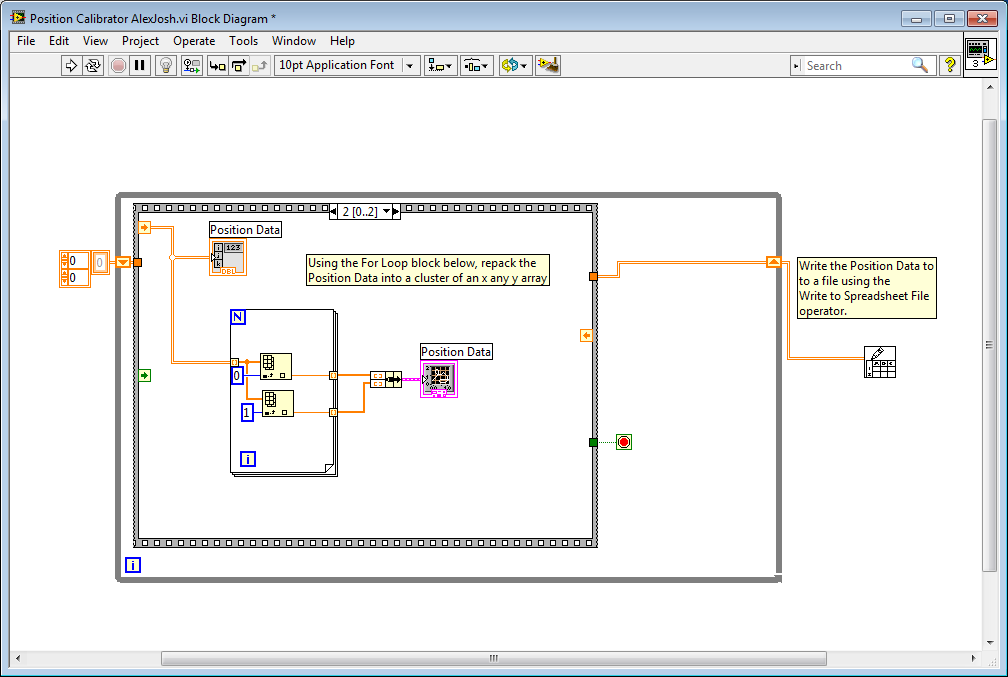
\includegraphics[scale = 0.3]{12c.PNG}
        \caption{Our Constructed Position Calibrator.vi \cite{lab11}}
        \label{fig:my_label}
    \end{figure}
    We ran the calibration routine, followed the calibration steps mentioned in the lab instructions, and yielded the following calibration data:
    \begin{table}[H]
        \centering
        \caption{Calibration Data Found from Using our Position Calibrator.vi}
        \label{my-label}
        \begin{tabular}{ll}
        \textbf{Number of Turns} & \textbf{Light Signal (V)} \\ \hline
        0.000 & 0.697 \\
        0.125 & 1.562 \\
        0.250 & 2.001 \\
        0.375 & 2.360 \\
        0.500 & 2.632 \\
        0.625 & 3.143 \\
        0.750 & 3.671 \\
        0.875 & 4.425 \\
        1.000 & 5.009 \\
        1.250 & 6.717 \\
        1.500 & 8.784 \\
        1.750 & 10.555
        \end{tabular}
        \end{table}

%13
\subsection{}
    We changed the setpoint of the levitator in 0.1mm steps, and found that the range by which the levitator could hold the ball is $\approx$0 to 1.7mm.\\\indent With the setpoint at 1.1mm, we added a time delay to increase the service time, and noticed that we could add at most a 3 ms delay to the service interval (call this the continuous delay) before the ball began to drop.\\\indent We added code that inserts a delay every time push a boolean control (call this the intermittent delay). We increased this delay to 30 ms before the ball began to drop.\\\indent The maximum tolerable continuous delay (3ms) is far less than the maximum tolerable intermittent delay (30ms) because of the integral term in the PID equation \cite{lab11}. We notice that the integral term is largely responsible for any "smoothing" out of time delays in the signal production, that is, if the levitator loses power/signal for a little bit due to time delay, the integral term sort of "saves" the information of the necessary response for a small period of time, kind of like how integrals are used to average out signals. As the intermittent delay increases to 30ms, we know that the integral term will still be finite as time passes and depends on the historical data of the driving signal. We see that this "saved" signal diminishes as time increases. In other words, once the signal is turned off then turned back on, the ball can return to its original position. However, with the continuous delay, the integral term slowly diminishes over a succession of delay cycles and as this occurs the ball is at a lower and lower height (does not have enough time to recover) until it completely drops; it is like losing stability over time each time the signal is shutoff (a hysteresis effect).  We would thus expect the max continuous time delay to be smaller than the max intermittent time delay. Lastly, we can assume (as a rule of thumb) that for PIDs \cite{lab11}, that they work well if their servicing time is 1/10 the time of an event, and we see below that the time it takes for the ball to fall out of its range is about 10ms. We see that the service time is 3ms (continuous time delay), which is a little less than 3/10 of the total event time. So we see that in this case, the PID/levitator should likely fail at this 3ms. And we see that the time it takes for the ball to fall out of range is at the same order of magnitude as the intermittent delay (30ms), which is reasonable because the during the intermittent delay, the ball is given the time to fall. Thus, we attain the difference between the two delays.
    \\\indent We calculate the  amount of time it takes for a ball to fall an appropriate amount of distance. Its setpoint is at 1.1mm, and its maximum range value is at 1.7mm. So the appropriate amount of distance before the ball falls is where it falls from its setpoint to its range, the distance of which is 0.6mm. This fall occurs in time (d is distance and g is acceleration due to gravity):
    \begin{equation}
        t = \sqrt{2*d/g} = \sqrt{\frac{2*0.6mm}{\frac{9.8m}{s^{2}}}} \approx 11.7 ms 
    \end{equation}
    The time it takes for the ball to fall this distance is on the same order of magnitude as the maximum tolerable continuous delay (3ms) and the maximum tolerable intermittent delay (30ms), suggesting the effects as aforementioned. 

%14
\subsection{}
    We took a look at the DAC output on the scope and denoted the excursion size as being the peak-peak amplitude of the signal (for a set point of 1.1mm). Below is a table depicting excursion size vs. proportional gain:
    \begin{table}[H]
        \centering
        \caption{Proportional Gain vs. Excursion Size}
        \label{my-label}
        \begin{tabular}{ll}
        \textbf{Proportional Gain} & \textbf{Amplitude/Excursion Size (V)} \\ \hline
        -2 & 1.4 \\
        -5 & 0.4 \\
        -10 & 0.8 \\
        -20 & 1.8 \\
        -30 & 2.5 \\
        -35 & 2.7
        \end{tabular}
        \end{table}
    We see for -10 gain, the excursion size is 800mV. We could make the magnitude of the proportional gain as high as 35 and as low as 2 without the ball falling. We restored the proportional gain. We then changed the derivative time and noticed the ball stayed under control between a $T_d$ of 10$\mu$s-500$\mu$s for a setpoint of 1.1mm. With set point of 1.1mm, we restored the derivative time and decreased the integral time to 0s. The ball still levitated, but did so at a new position of 1.35mm, a change in vertical distance of 0.25mm from the original setpoint position.

%15
\subsection{}
    With "Impulse Response.vi" (new set point of 1mm) we varied the derivative time over which the ball stayed levitating. We saw that the lowest derivative time was 20$\mu$s and the largest time was 190$\mu$s. We noticed that at various $T_d$ levels, the ball would exhibit underdamping, overdamping, and critical damping behaviors after being dropped a little. We note that at critical damping, the time it takes for the system to stabilize is lowest. Displayed below is a table showing derivative times $T_d$ vs. stabilization time of the system:
    \begin{table}[H]
        \centering
        \caption{Derivative Time versus Stabilization Time of Impulse Response}
        \label{my-label}
        \begin{tabular}{ll}
        \textbf{$T_d$ ($\mu$s)} & \textbf{Stabilization Time (ms)} \\ \hline
        30 & 230 \\
        50 & 140 \\
        90 & 160 \\
        110 & 150 \\
        150 & 190 \\
        190 & 180
        \end{tabular}
        \end{table}
    We see that at $T_d$ of 50 ms, the ball appears to be critically damped as the stabilization time is the lowest. We also noticed that our ball began to oscillate at around 30ms leading to the increase in stabilization time as seen above. 




\section{Signature Page}
\begin{figure}[H]
    \centering
    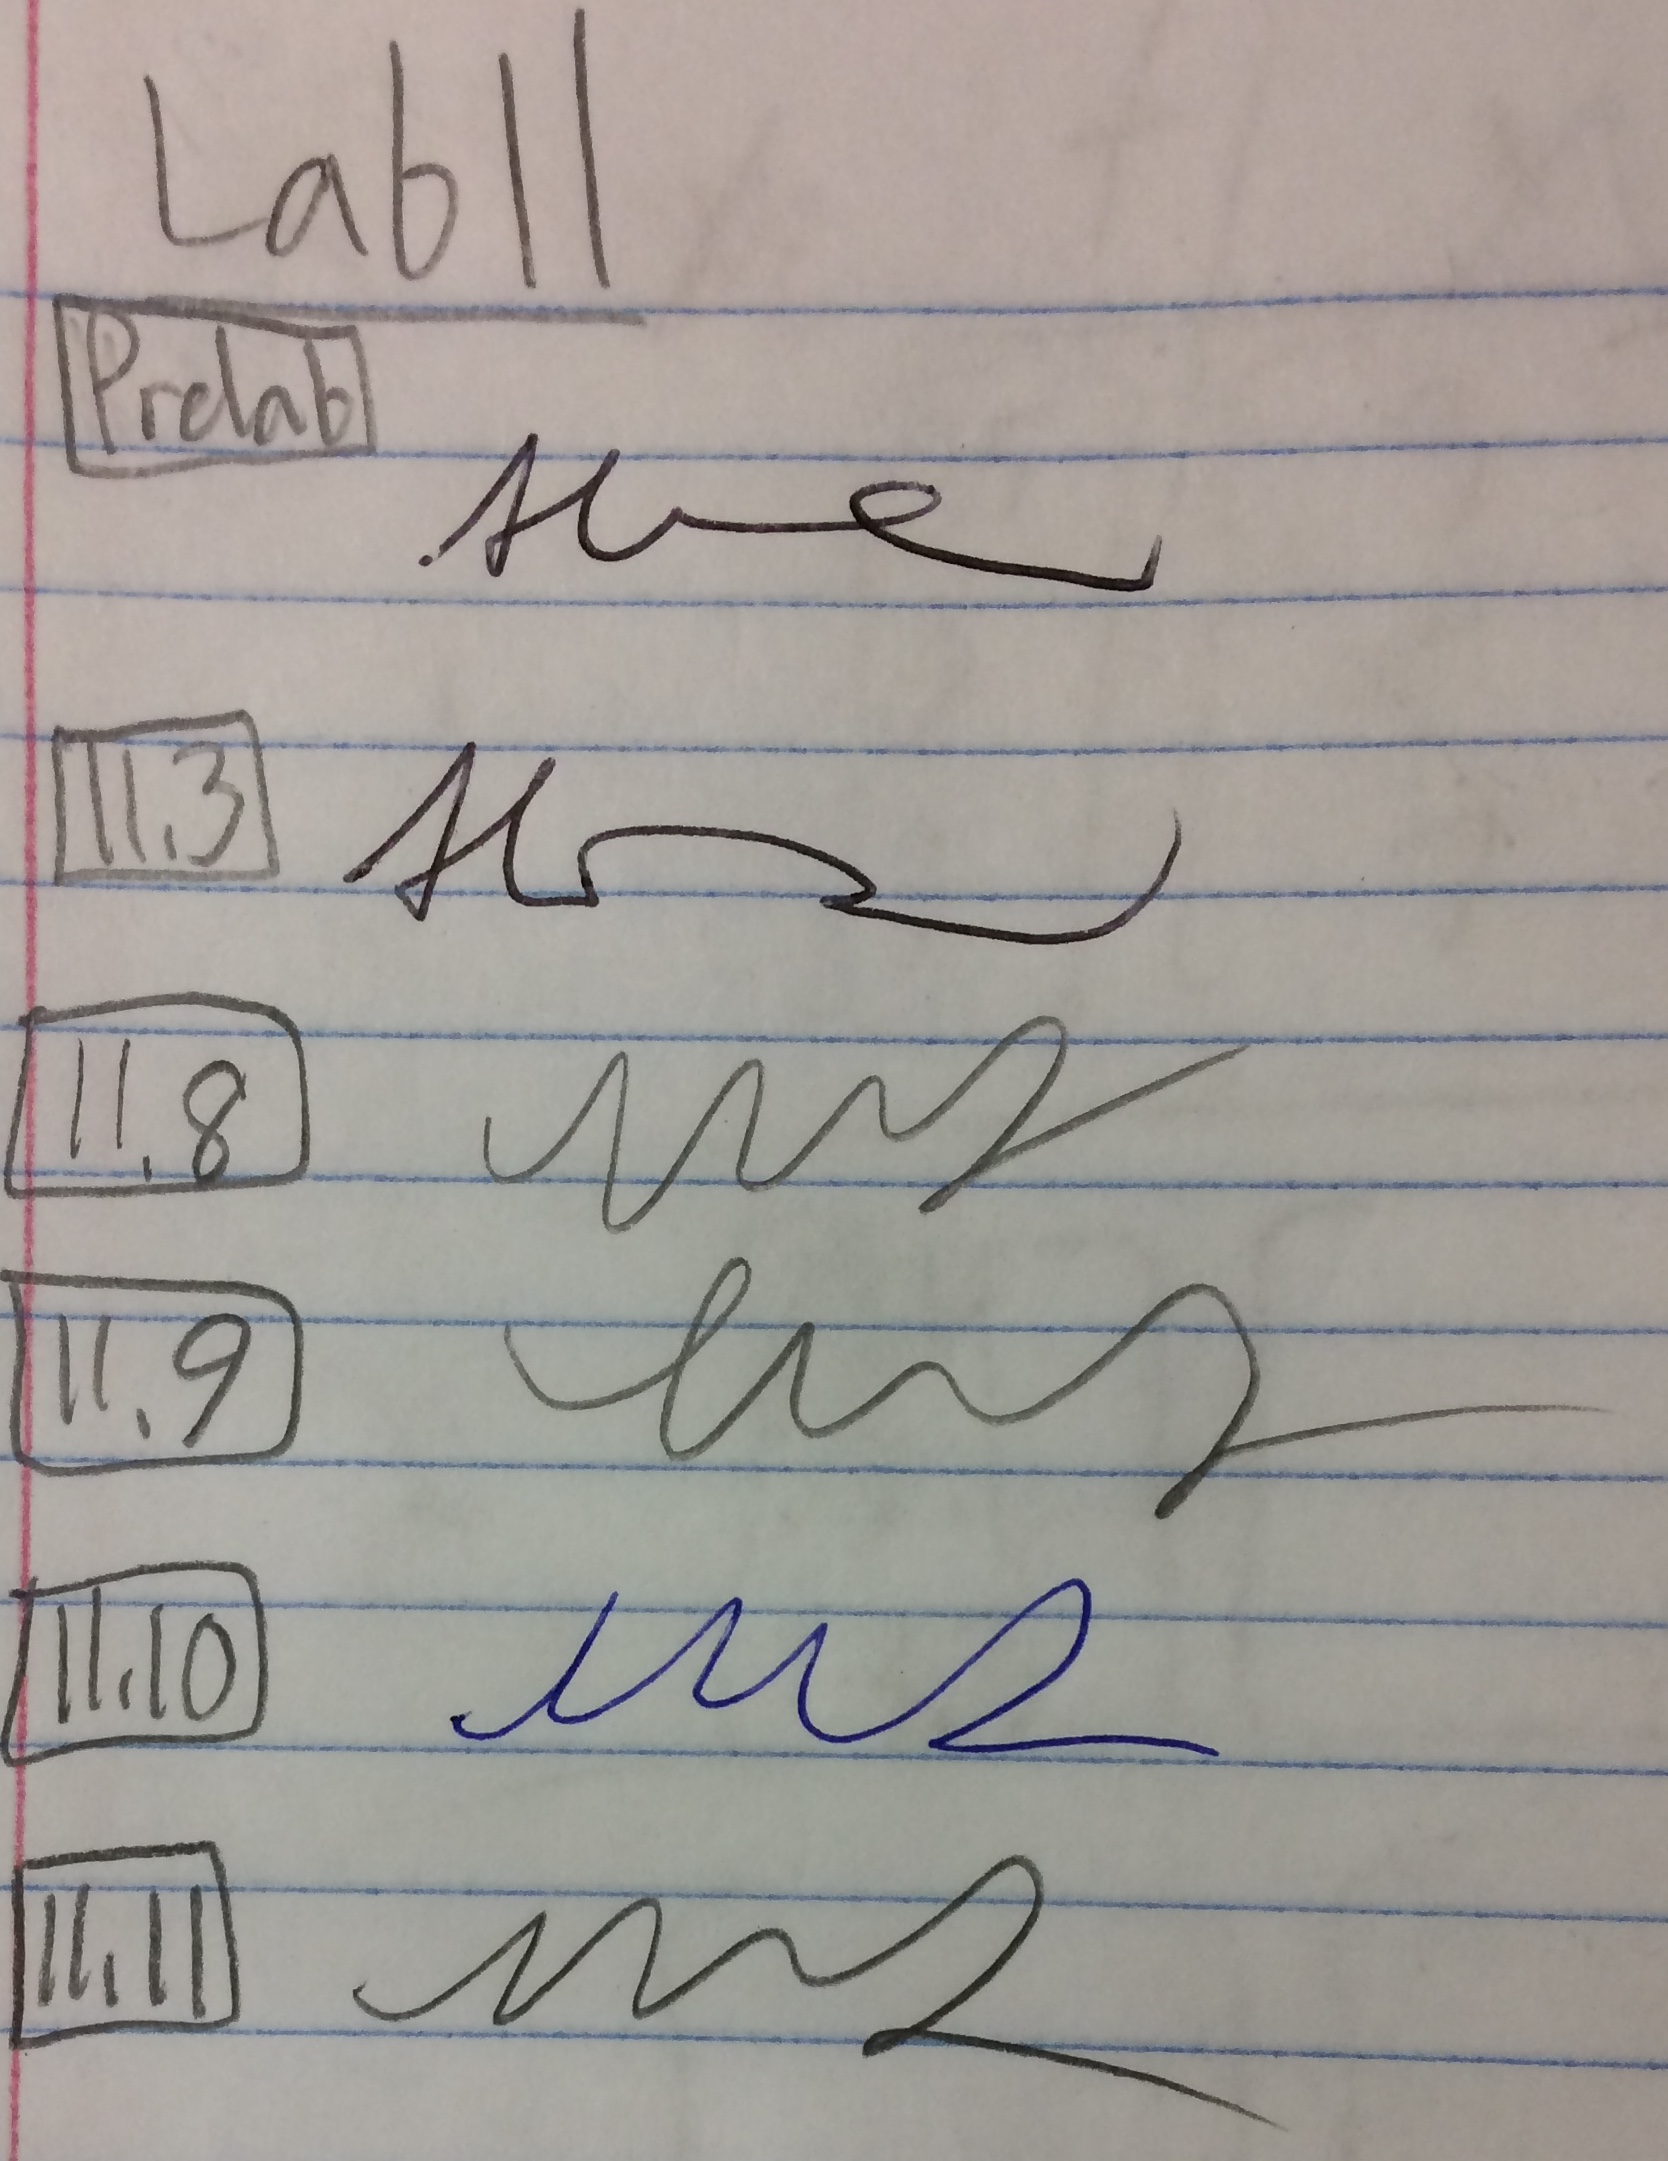
\includegraphics[scale = 0.15]{sig.jpg}
    \caption{Signatures}
    \label{fig:my_label}
\end{figure}



\bibliography{joshbib}{}
\bibliographystyle{plain}


\end{document}

\begin{figure}[H]
    \centering
    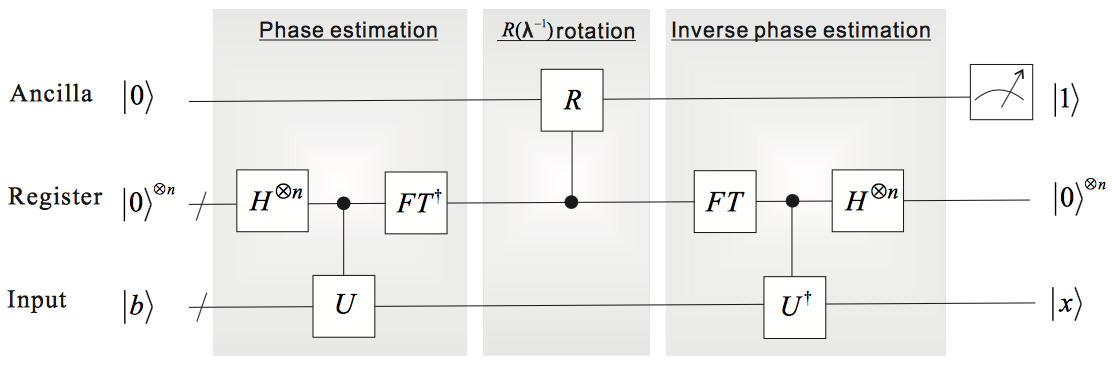
\includegraphics[scale = 0.5]{1.png}
    \caption{Caption \cite{lab11}}
    \label{fig:my_label}
\end{figure}
